\label{sec:appen}
Durante l'analisi descritta nella sezione \ref{sec:aba} vengono rappresentati i due istogrammi della carica degli eventi classificati muoni nel CD e nel WP attraverso il metodo di correlazione temporale. Di seguito si possono osservare i diversi spettri di carica della Water Pool al variare del tempo di correlazione  (da $10\,\unit{ns}$ a $1000\,\unit{ns}$).
\label{sec:app1}
\begin{figure}[h!]
    \centering
    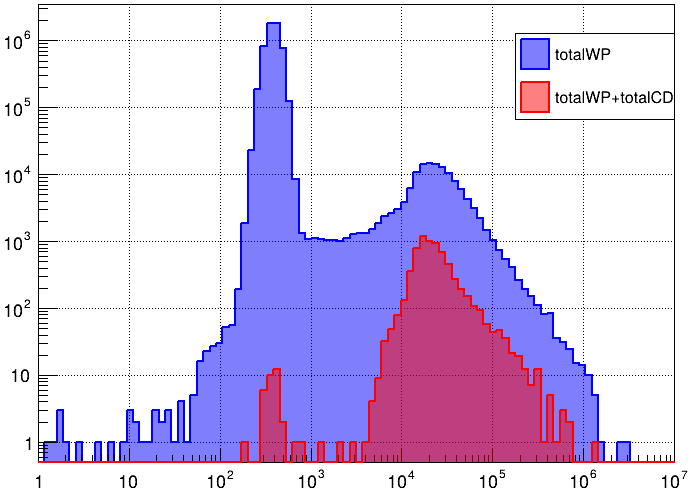
\includegraphics[width=0.4\textwidth]{Appendice/WP_RUN4049_tolerance_10.00.png}
    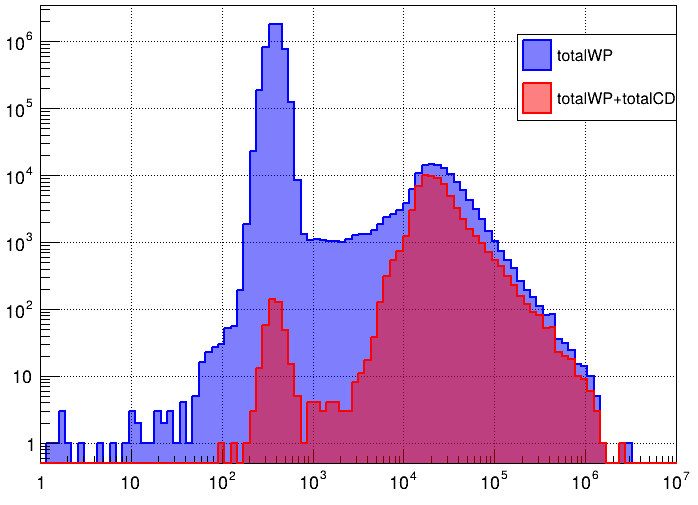
\includegraphics[width=0.4\textwidth]{Appendice/WP_RUN4049_tolerance_100.00.png}
    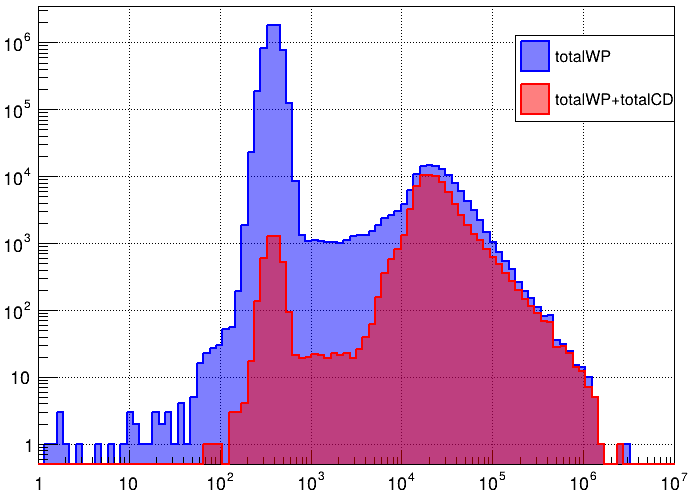
\includegraphics[width=0.4\textwidth]{Appendice/WP_RUN4049_tolerance_1000.00.png}
    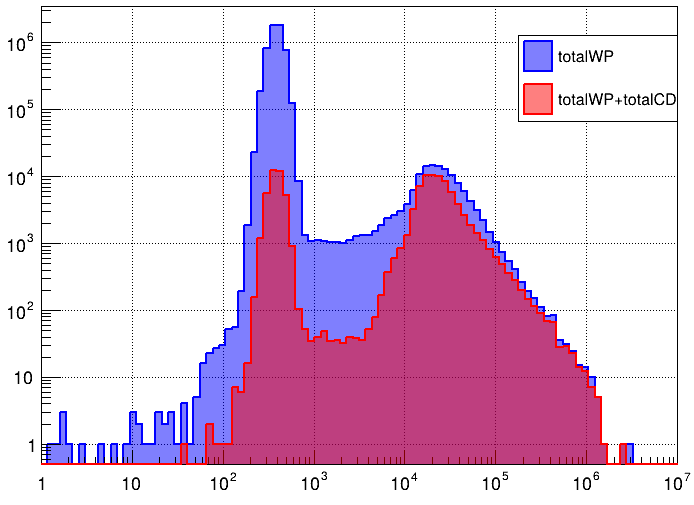
\includegraphics[width=0.4\textwidth]{Appendice/WP_RUN4049_tolerance_10000.00.png}
    \caption{In questa figura si può apprezzare l'effetto della variazione del tempo di tolleranza sullo spettro WP degli eventi totali e degli eventi correlati temporalmente.}
    \label{Fig:graficiWP}
\end{figure} 